%%%%%%%%%%%%%%%%%%%%%%%%%%%%%%%%%%%%%%%%%%%%%%%%%%%%%%%%%%%%%%%%%%%%%%%%%%%%%%%%%%%%%%%%%%%%%%
% Template Beamer Sugestivo para Projetos no Senac
% by ezefranca.com
% Based on MIT Beamer Template
% As cores laranja e azul seguem o padrao proposto no manual de uso da identidade visual senac
%%%%%%%%%%%%%%%%%%%%%%%%%%%%%%%%%%%%%%%%%%%%%%%%%%%%%%%%%%%%%%%%%%%%%%%%%%%%%%%%%%%%%%%%%%%%%% 

\def\leq{\leqslant} % eleganter \leq-symbool  
\def\geq{\geqslant} % eleganter \geq-symbool  

%\documentclass{beamer} %voce pode usar este modelo tambem
\documentclass[handout,t]{beamer}
\usepackage{graphicx,url}
  
\usepackage[utf8]{inputenc}

 
\batchmode
% \usepackage{pgfpages}
% \pgfpagesuselayout{4 on 1}[letterpaper,landscape,border shrink=5mm]
\usepackage{amsmath,amssymb,enumerate,epsfig,bbm,calc,color,ifthen,capt-of}
\usetheme{Berlin}
\usecolortheme{senac}

%-------------------------Titulo/Autores/Orientador------------------------------------------------
\title[Final Project]{Understanding GDP per Capita }
\date{}
\author{Daniel Ocampo \& Jeremy Moore}

%-------------------------Logo na parte de baixo do slide------------------------------------------
\pgfdeclareimage[height=0.7cm]{senac-logo}{images.png}
\logo{\pgfuseimage{senac-logo}\hspace*{0.5cm}}

%-------------------------Este código faz o menuzinho bacana na parte superior do slide------------
\AtBeginSection[]
{
  \begin{frame}<beamer>
    \frametitle{Outline}
    \tableofcontents[currentsection]
  \end{frame}
}
\beamerdefaultoverlayspecification{<+->}
% -----------------------------------------------------------------------------
\begin{document}
% -----------------------------------------------------------------------------

%---Gerador de Sumário---------------------------------------------------------
\frame{\titlepage}
\section[]{}
\begin{frame}{Summary}
  \tableofcontents
\end{frame}
%---Fim do Sumário------------------------------------------------------------


% -----------------------------------------------------------------------------
\section{Movtivation}
\begin{frame}{Introdcution}
%introducao
\begin{itemize}
\item Entrepreneurship
\item Economics 
\item GDP
\item Successful Business 
\end{itemize}

\begin{figure}
    \centering
    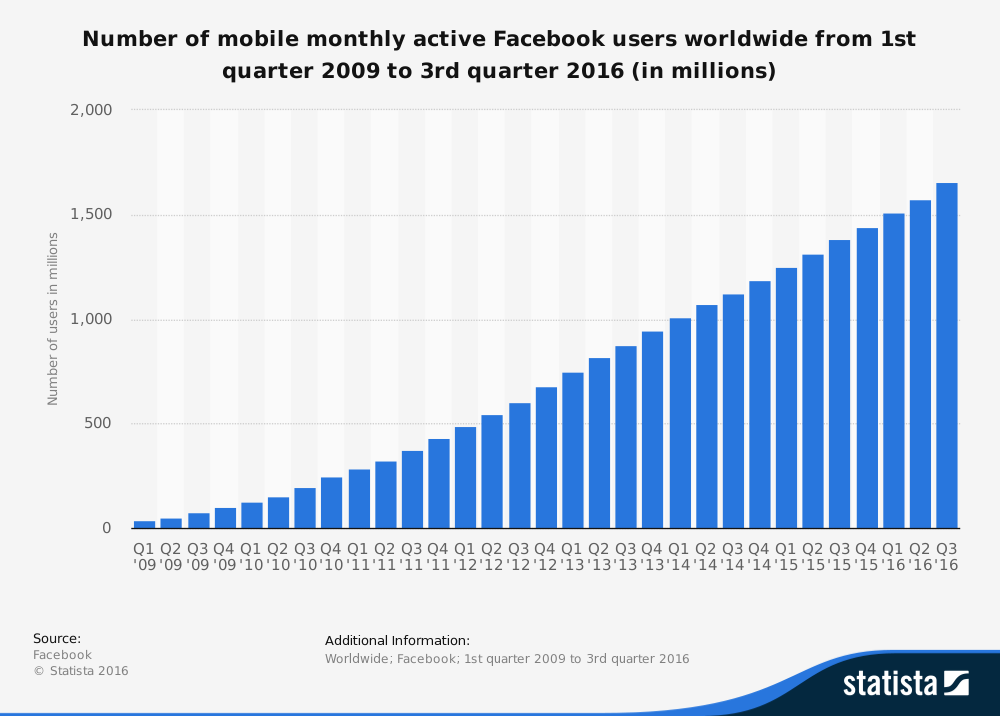
\includegraphics[width = 0.45\textwidth]{facebook}
    \caption{Facebook users}
  \end{figure}



\end{frame}
%------------------------------------------------------------------------------

%------------------------------------------------------------------------------
\section{Related Work}
\begin{frame}{Related Work}
\begin{itemize}
\item User who used phones for 2 hours longer had higer chances of lower back pain
\item Attention span is now down to 8 seconds 
\item Less hours of sleep
\item User look at phone before bed 

\begin{figure}
    \centering
    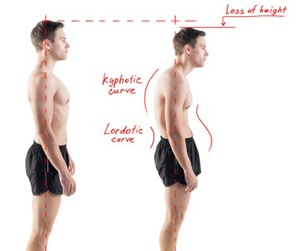
\includegraphics[width = 0.35\textwidth]{back}
    \caption{User and back pain}
  \end{figure}

\end{itemize}
\end{frame}
%------------------------------------------------------------------------------

%------------------------------------------------------------------------------
\section{Mobile Applications}
\begin{frame}{Mobile application}
\begin{itemize}
\item Andriod Studio
\item Tasker, App Inventor
\item Pros   
\item Cons
\end{itemize}

\begin{figure}
    \centering
    
\includegraphics[width = 0.35\textwidth]{studio}
    \caption{Creation of mobile applications }
  \end{figure}

\end{frame}
%------------------------------------------------------------------------------

%------------------------------------------------------------------------------
\section{Databases}
\begin{frame}{Databases}
%consideraçoes e resultados
\begin{itemize}
\item Sqlite3
\item Queries 
\item Analysis
\end{itemize}

\begin{figure}
    \centering
    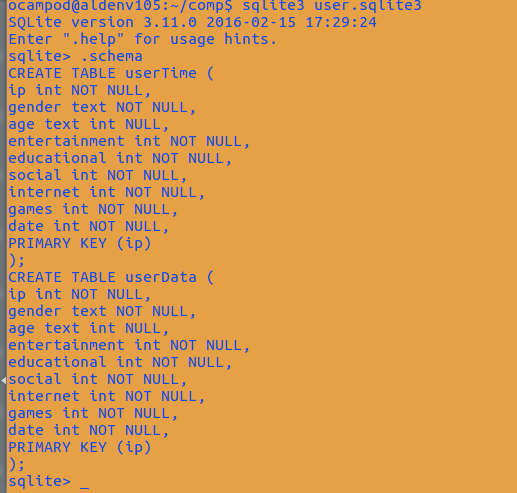
\includegraphics[width = 0.35\textwidth]{terminal}
    \caption{Creation of mobile applications }
  \end{figure}


\end{frame}
%------------------------------------------------------------------------------

%------------------------------------------------------------------------------
\section{Application Study}
\begin{frame} 
\begin{itemize}
   \item Survey Collect Data 
  \item Create Mobile Application
  \item Collect data
  \item Return data (visual) 
  \item Store data 
  \item Analyze data
 \end{itemize} 
 
 
 \begin{figure}
    \centering
    \includegraphics[width = 0.34\textwidth]{gram}
    \caption{Steps taken }
  \end{figure}
      
    \end{frame}
%------------------------------------------------------------------------------

%------------------------------------------------------------------------------
\section{Back up plan}
\begin{frame}{Back up Plan}
\begin{itemize}
\item Tasker 
\item App Inventor 
\item Tablets 
\item Participants 
\end{itemize}

\end{frame}
%------------------------------------------------------------------------------

%------------------------------------------------------------------------------
\section{Future work}
\begin{frame}{Future Work}

  \begin{itemize}
    \item Filters 
    \item Fitbit
    \item Constant checking 
  \end{itemize}
 
 


  
\end{frame}




 \section{Conclustion}
 \begin{frame}{Conclustion}
 \begin{itemize}
  \item Problems 
 \item Possible soultion 
 \item Reasons 
 \end{itemize}

 \end{frame}
 
%------------------------------------------------------------------------------

% -----------------------------------------------------------------------------
\end{document}
%-----------------------------------------------Este comentario nunca aparecera